\documentclass{report}

% Language setting
\usepackage[main=portuguese, english]{babel}
\usepackage{csquotes}

% Set page size and margins
\usepackage[a4paper,top=2cm,bottom=2cm,left=3cm,right=3cm,marginparwidth=1.5cm]{geometry}

% Useful packages
\usepackage{ulem}
\usepackage{parskip}
\usepackage{indentfirst}
\usepackage{setspace}
\usepackage{amsmath}
\usepackage{array}

\usepackage{graphicx}
\usepackage{xcolor}
\usepackage{colortbl}
\usepackage{subfigure}
\usepackage{titlesec}
\usepackage[colorlinks=false, allbordercolors={0 0 0}, pdfborderstyle={/S/U/W 0.25}]{hyperref}
\usepackage[hypcap=true]{caption}
\usepackage{enumitem}
\usepackage{soul}
\usepackage{ragged2e}

\usepackage[backend=biber,]{biblatex}
\addbibresource{reference.bib}

% Set section numbering from 1.1
\renewcommand{\thesection}{\arabic{section}.1}
\newcolumntype{P}[1]{>{\centering\arraybackslash}p{#1}}
\newcolumntype{M}[1]{>{\centering\arraybackslash}m{#1}}

\let\oldsection\section
\renewcommand\section{\clearpage\oldsection}

% Change section formatting
\titleformat{\section}
  {\fontsize{12}{15}\selectfont\bfseries}{\thesection}{1em}{}

% Configure indentations
\setlength{\parindent}{1.5cm}

\begin{document}

    \begin{titlepage}
        \centering
        
        \LARGE {Universidade Federal do Rio Grande do Sul \\ Instituto de Informática}
    
        \begin{figure}[h!]
        \centering
        \subfigure
        {
\includegraphics[width=0.35\linewidth]{images/logos/UFRGS.png}}
        \hspace{1cm}
        \subfigure
        {
\includegraphics[width=0.35\linewidth]{images/logos/INF.png}}
        \end{figure}
    
        \LARGE {INF01017 \\ Aprendizado de Máquina}
        
        \vfill
        {\noindent\hrulefill \\
        \bfseries \Huge{Trabalho Prático Final} \\ \LARGE{Predição de consumo de combustível utilizando aprendizado de máquina} \\
        \noindent\hrulefill}
        
        \vfill
        {\LARGE Luís Filipe Martini Gastmann (00276150) \\ Pedro Lubaszewski Lima (00341810) \\ Vinícius Boff Alves (00335551) \\~\\ Turma U}
    
        \vfill
        {\LARGE 9 de novembro de 2024}
        
    \end{titlepage}

        \renewcommand{\contentsname}{Sumário}
        \tableofcontents
        \clearpage
        \addtocontents{toc}{\protect\thispagestyle{empty}}

\section{Definição do Problema e Coleta de Dados}

O objetivo deste trabalho é prever o consumo médio de combustível de um carro através de algumas das suas características e origens de fabricação.
Alguns atributos das instâncias são a marca, a quantidade de cilíndros, o porte do veículo etc.

O conjunto de dados utilizado para desenvolver este trabalho foi obtido da seguinte página do Kaggle:
\href{https://www.kaggle.com/datasets/arslaan5/explore-car-performance-fuel-efficiency-data}{Explore Car Performance: Fuel Efficiency Data}.
Essa tarefa contará com diversas técnicas de preparação dos dados para posteriormente iniciar a seleção e
avaliação de modelos para essa tarefa.

\section{Análise Exploratória e Pré-processamento dos Dados}

\subsection{Análise Exploratória dos Dados}

Este \textit{dataset} possui 550 instâncias, com 11 atributos preditores e 1 atributo alvo. Esse último torna a tarefa dos modelos em regressão,
visto que o objetivo aqui é prever o consumo médio de combustível de carros. No conjunto de dados, esse atributo predito se chama \textit{combination mpg}.

Dos atributos preditores, observa-se que há 5 atributos numéricos (\textit{city mpg}, \textit{cylinders}, \textit{displacement}, \textit{highway mpg} e \textit{year}).
Além deles, os 6 atributos restantes são categóricos: \textit{class}, \textit{drive}, \textit{fuel type}, \textit{make}, \textit{model} e \textit{transmission}.
Com isso em mente, criou-se alguns gráficos para analisar correlações e distribuições dos dados. A seguir, o \textit{violin plot}
do atributo alvo pelo número de veículos:

\begin{figure}[h!]
  \centering
  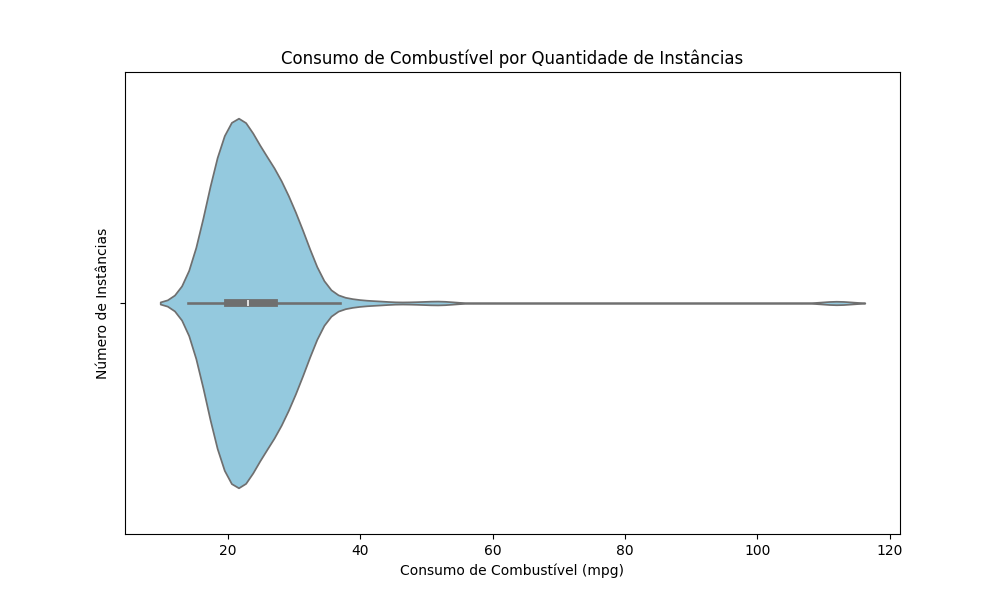
\includegraphics[width=.85\linewidth]{images/plots/violin_plots/pure_combination_mpg.png}
  \caption{\label{img:combination_dist} \textit{Violin Plot} de Consumo Médio}
\end{figure}

Nesse ponto, já se observa que há instâncias problemáticas, claramente \textit{outliers} que devem ser removidas do conjunto de dados. Ademais, a maior concentração dos veículos
apresenta consumo médio entre 15 e 30mpg, algo que pode guiar bastante os modelos. Após isso, analisou-se o atributo de classes de veículos para ter uma ideia da sua distribuição
em um gráfico de setores.

\begin{figure}[h!]
  \centering
  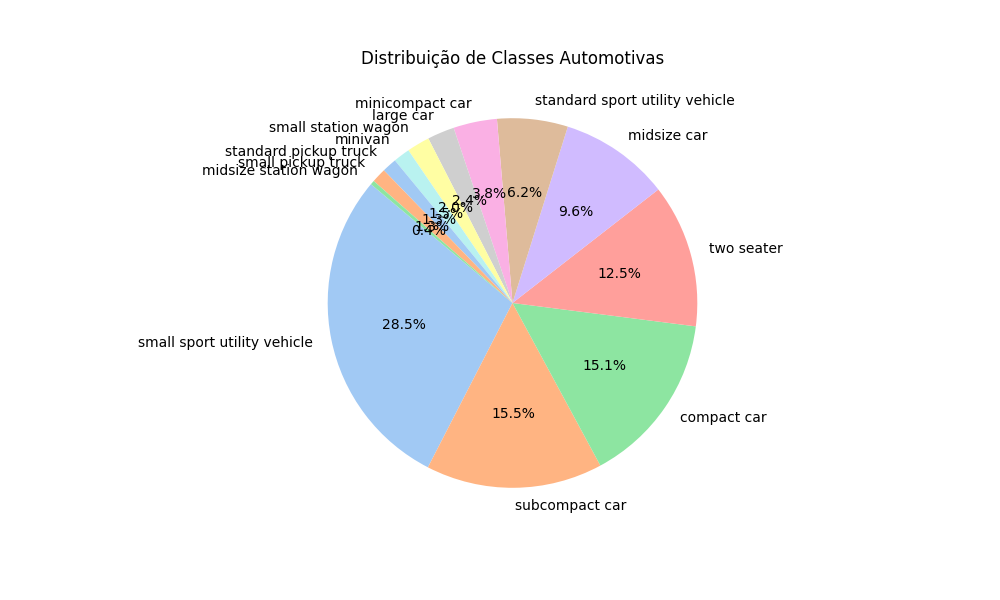
\includegraphics[width=.85\linewidth]{images/plots/pie_charts/pure_car_classes.png}
  \caption{\label{img:classes_dist} Distribuição de Classes de Veículos}
\end{figure}

Com ele, é perceptível que talvez seja necessário agrupar as classes de veículos e outros atributos que contenham classes com muito poucos representantes, como \textit{midsize station wagon},
por exemplo, em uma classe geral chamada \textit{others}. Porém, essa discussão será retomada na \autoref{subsec:revisit_pre}. No entanto, algo que é necessário é a codificação dos
atributos categóricos em numéricos para padronizar a entrada numérica dos modelos.

Por fim, analisou-se a Correlação de Pearson entre os atributos numéricos através do \textit{heatmap} abaixo:

\begin{figure}[h!]
  \centering
  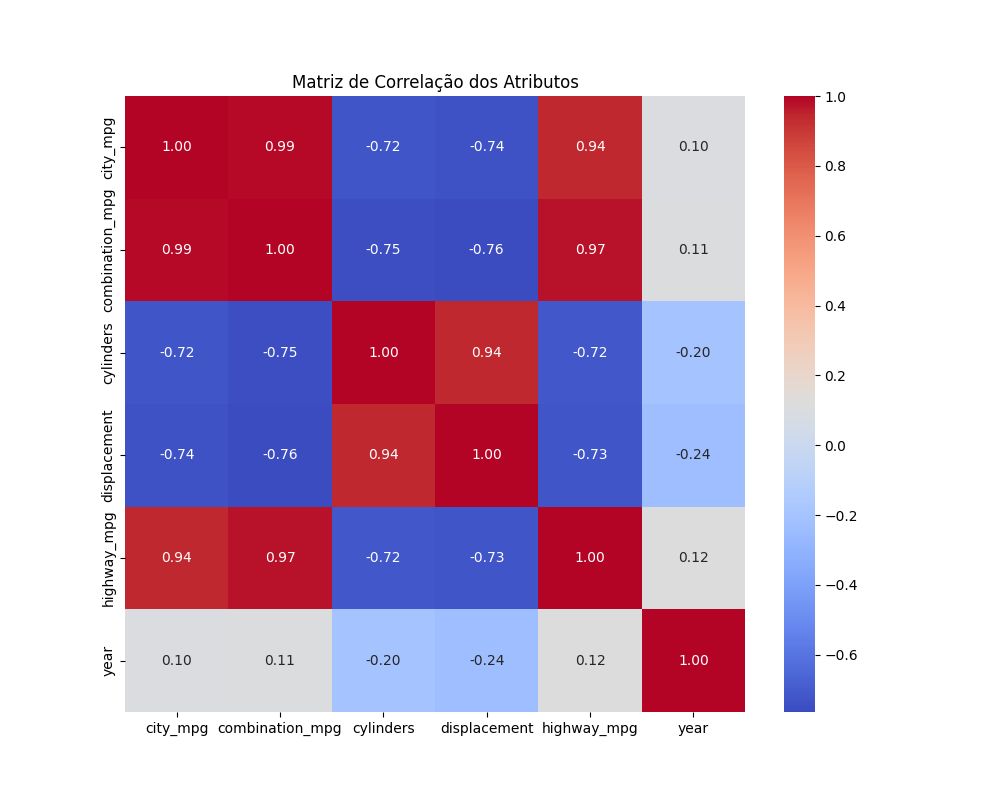
\includegraphics[width=.85\linewidth]{images/plots/heatmaps/numeric_atributes_correlation.png}
  \caption{\label{img:num_heatmat} \textit{Heatmap} de Correlações entre Atributos Numéricos}
\end{figure}

Olhando para o gráfico acima, percebe-se que há diversos atributos preditores que apresentam alto nível de correlação com a saída \textit{combination mpg} e entre si. Ambos os atributos
\textit{highway mpg} e \textit{city mpg} serão descartados do \textit{dataset} por terem alta correlação entre si e com o valor da saída do modelo, facilitando demais a tarefa dos modelos.
Além disso, observa-se que \textit{displacement} e \textit{cylinders} também apresentam alta correlação entre si. No entanto, a informação de \textit{cylinders} ou cilindros de um carro é diferente
da informação de \textit{displacement} ou cilindradas desse. As cilindradas representam o volume total dos cilindros de um motor. Por conta disso, são calculados a partir dos cilindros, porém
acrescentam um dado a novo ao problema. Ou seja, vale a pena mesmo assim manter ambos os atributos no \textit{dataset}.

Isto não foi ilustrado pelos gráficos, porém os dados numéricos apresentam diversas escalas diferentes, exigindo técnicas de normalização após a separação de conjuntos de treinamento/validação
e de testes.

\subsection{Pré-processamento dos Dados} \label{subsec:pre-proc-de-dados}

Como já discutido na seção acima e analisando alguns trabalhos realizados com esse conjunto de dados, esses sendo de Lunovian \cite{Lunovian}, da Ayşe \cite{Ayşe} e do Priyanshu \cite{Priyanshu},
implementou-se algumas estratégias de pré-processamento nos dados deste problema.

Primeiramente, realizou-se a remoção dos atributos discutidos anteriormentes. Esses sendo o \textit{highway mpg}, \textit{city mpg} e \textit{displacement}, visto que apresentam alto níveis de
correlação entre si e com o valor da saída do modelo. Após essa remoção, filtrou-se as instâncias com muitos atributos faltantes (em geral, carros elétricos que funcionam diferentemente dos carros
que funcionam com combustíveis fósseis).

Depois disso, foi realizada a limpeza de instâncias cujo atributo alvo representava um \textit{outlier} no gráfico de distribuição de consumo médio dos veículos. Essa estratégia é necessária para
evitar que os modelos sejam treinados com instâncias que não representam bem a grande a maioria dos veículos. Utilizou-se a medida padrão de 1.5 vezes o IQR para identificar \textit{outliers}.

Sobre a codificação dos atributos, o grupo utilizou a codificação padrão de categórico para numérico que é o \textit{one-hot encoding}. A justificativa para isso é que os atributos categóricos não
apresentam nenhuma ordem específica que justifique utilizar uma codificação em números inteiros. Além disso, em relação à normalização, baseado no trabalho do Jason Brownlee \cite{ColumnTransformer} e
do Matheus Vasconcelos \cite{PadronizarDados}, optou-se por utilizar a padronização por \textit{min-max}, visto que é uma normalização mais eficaz na maioria dos casos, não exigindo uma distribuição normal
dos dados. Tanto a codificação, quanto a normalização foram aplicadas após a separação de conjuntos de treinamento/validação e de testes separamente (evitando vazamento de dados).

Um outro problema encontrado consiste na possibilidade de não ser visto algum modelo de carro (\textit{model}) no treinamento. Isso pode acontecer pois há uma quantidade muito grande de modelos diferentes,
alguns deles com poucas instâncias. Para solucionar esse problema, ``forçou-se" a haver pelo menos uma instância de cada modelo de veículo no conjunto de treinamento, antes de realizar a separação de
conjunto de dados para teste. Para realizar essa última separação, utilizou-se a função \texttt{train\_test\_split()} com um \texttt{test\_size} de 15\%. Essa ação corresponde à estragégia de \textit{holdout}
vista em aula para a primeira divisão dos dados.

\section{Abordagem, Algoritmos e Estratégias de Avaliação}

Seguindo as ideias discutidas nos ítens anteriores, este problema consiste em uma tarefa de regressão. Por conta disso, o grupo buscou no conteúdo programático da disciplina algoritmos para essa tarefa.
Com isso, separou-se os seguintes algoritmos de aprendizado para serem avaliados: \textbf{\textit{k-Nearest Neighbors}}, \textbf{\textit{Random Forest}}, \textbf{Regressão Linear}, \textbf{Redes Neurais}
e \textbf{SVM}. A escolha desses modelos também foi inspirada nos trabalhos de Neslihan Avsar \cite{LinearRegression}, de James McCaffrey \cite{Regression} e de isitapol2002 \cite{MultRegression}.

Definidos esses algoritmos e as estratégias de pré-processamento, definiu-se como estratégia de validação desses algoritmos o \textit{k-fold cross-validation}. Essa é a \textit{magnum opus} das estratégias
de validação de aprendizado supervisionado, então foi a adotada pelo grupo. O valor de \texttt{k = 13} foi definido experimentalmente. A justificativa mora na quantidade de instâncias que
sobraram para a validação após a separação de modelos de carros únicos para o treinamento e do conjunto de testes. O número final de elementos por \textit{fold} beira 18 instâncias (quantidade não muito grande,
porém proporcionalmente aceita para a quantidade total de instâncias do \textit{dataset}), gerando 13 medições de erro para cada modelo.

Em cada iteração do \textit{k-fold cross-validation}, realizou-se a normalização e a codificação dos atributos correspondentes através dos métodos adequados do \texttt{scikit learn}. Foi fixada um \texttt{random\_state = 42}
para padronizar os resultados dos testes. Os hiperparâmetros utilizados nesta etapa foram todos os padrões de cada modelo da biblioteca do \texttt{scikit learn}.

A métrica de avaliação utilizada foi o \textit{Mean Squared Error} (MSE). O grupo optou por sumarizar os resultados do \textit{spot-checking} com apenas esta métrica (descartando o \textit{Mean Absolute Error}) porque são métricas
de natureza muito similar, já foi realizada a limpeza de \textit{outliers} que poderiam prejudicar os resultados dessas medições e essa é uma métrica que apresenta convergência mais rápida (Nirajan Acharya \cite{MSEAndMAE}). Além
disso, foram feitas diversas representações dessa métrica para obter maior confiança nos resultados obtidos.

\section{\textit{Spot-checking} de Algoritmos} \label{sec:spot_checking}

\subsection{Revisitando os Dados após o Pré-processamento}
\label{subsec:revisit_pre}

Com toda a metodologia explicada, voltar-se-á ao conjunto de dados pré-processados para realizar uma breve revisão dos dados de treinamento/validação. Primeiramente, após a remoção de \textit{outliers}, redução de dimensionalidade
e exclusão de instâncias de carros elétricos, gerou-se o seguinte gráfico de distribuição da saída a ser predita:

\begin{figure}[h!]
  \centering
  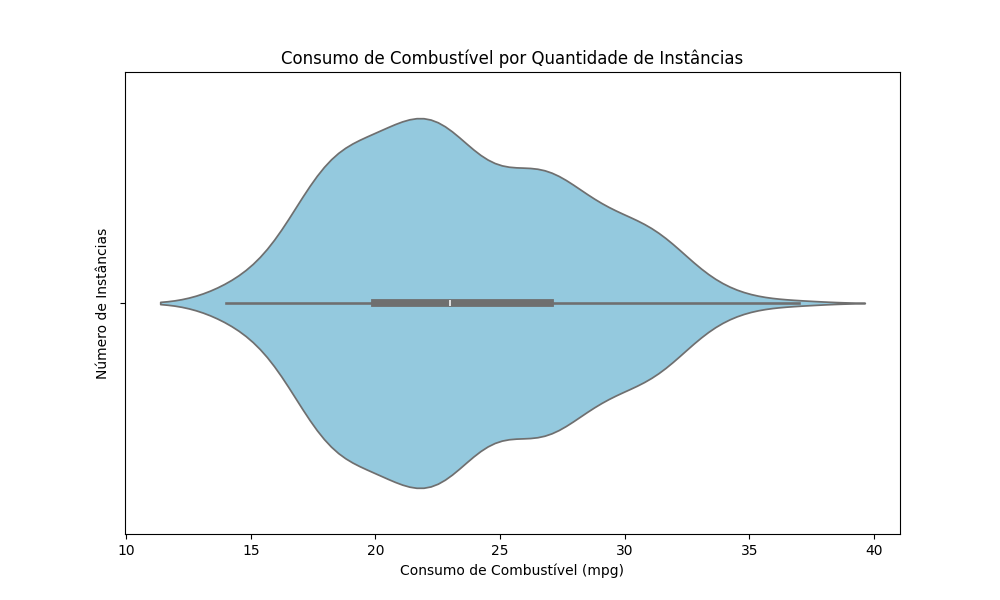
\includegraphics[width=.85\linewidth]{images/plots/violin_plots/no_outliers_combination_mpg.png}
  \caption{\label{img:pre_combination_dist} \textit{Violin Plot} de Consumo Médio Pré-processado}
\end{figure}

Agora observa-se que os dados quase se distribuem em formato de uma gaussiana. Além disso, continua observando-se a concentração de dados entre 15 e 30mpg de consumo médio. O gráfico de correlação também é refeito a seguir:

\begin{figure}[h!]
  \centering
  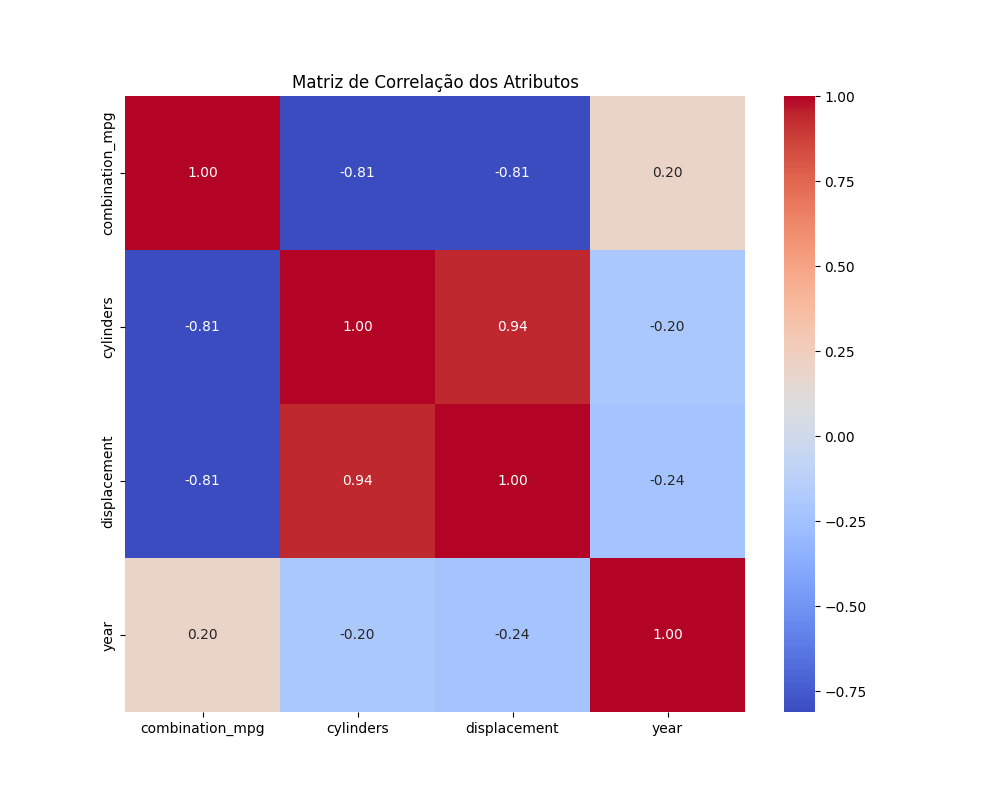
\includegraphics[width=.85\linewidth]{images/plots/heatmaps/no_outliers_numeric_atributes_correlation.png}
  \caption{\label{img:pre_num_heatmat} \textit{Heatmap} de Correlações entre Atributos Numéricos Pré-processados}
\end{figure}

Com a remoção dos atributos citados anteriormente, observa-se uma boa redução na correlação entre os atributos numéricos restantes. Algo que ajuda bastante a evitar a maldição da dimensionalidade.

Sobre a questão do agrupamento de atributos categóricos muito esparsos, foi percebido que o desempenho já nesta etapa se tornou inferior quando aplicado o agrupamento em comparação com o desempenho atingido
sem a aplicação desse pré-processamento (resultados com média aproximada de 1,5 e desvio padrão 0,5 de MSE passaram a mostrar resultados de mais de 2,5 de média e desvio padrão de mais de 1). Por conta disso,
optou-se por não adotar essa técnica para este problema.

\subsection{Sumarização dos Resultados}

Com esses dados revisitados, a seguir seguem os resultados obtidos pelos modelos:

\begin{table}[h!]
  \centering
  \begin{tabular}{| c | c | c |}
      \hline
      \rowcolor{lightgray}
      \textbf{Modelo} & \textbf{Média dos MSE} & \textbf{Desvio Padrão dos MSE} \\
      \hline
      kNN & 3,3227 & 1,3120 \\
      \hline
      \textit{Random Forest} & 1,8084 & 1,0998 \\
      \hline
      Regressão Linear & 1,4442 & 0,5086 \\
      \hline
      Redes Neurais & 1,1889 & 0,4046 \\
      \hline
      SVM & 3,9311 & 1,6636 \\
      \hline
  \end{tabular}
  \caption{\label{table:model_summary} Médias e Desvios Padrões dos MSE}
\end{table}

\begin{figure}[h!]
  \centering
  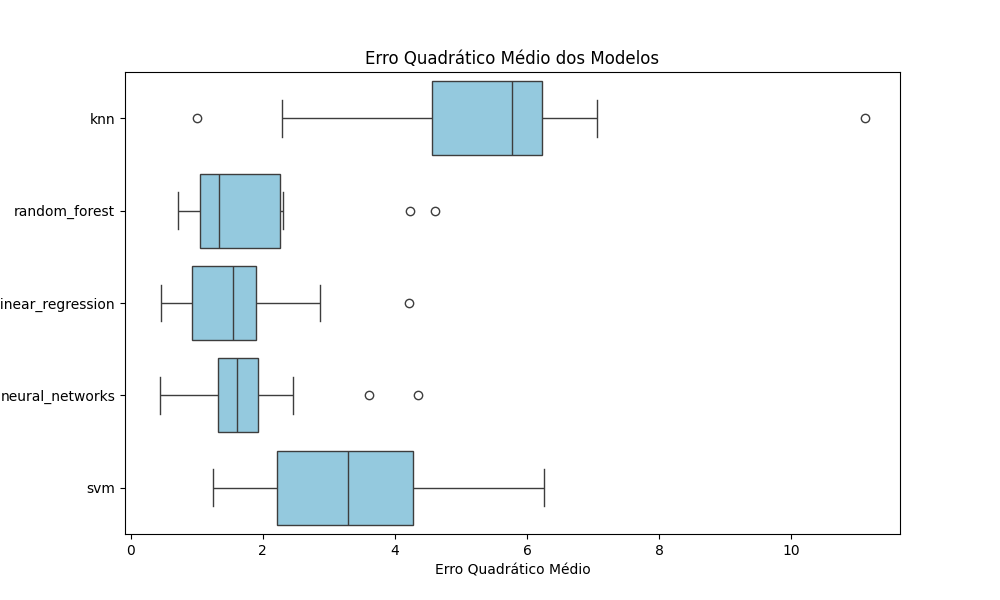
\includegraphics[width=.85\linewidth]{images/plots/box_plots/mse.png}
  \caption{\label{img:mse_boxplot} \textit{Box Plot} dos MSE}
\end{figure}

Por fim, com esses resultados, mesmo que os resultados não sejam reproduzíveis exatamente com os mesmos valores a cada vez que o código é executado, fica claro que os 3 modelos mais promissores foram
a \textbf{\textit{Random Forest}}, a \textbf{Regressão Linear} e as \textbf{Redes Neurais}. Como nenhum atributo foi otimizado, pode ser que os outros dois modelos se desempenhassem melhor, porém, com
as configurações básicas de hiperparâmetros, esses foram os três mais promissores.

Dentre esses, fica claro que os mais eficientes nesta tarefa foram o algoritmo de Regressão Linear e o modelo de Redes Neurais, visto que os erros da \textit{Random Forest} são mais elevados no geral quando
comparado com esses últimos dois. Mesmo que as Redes Neurais apresentem média e desvio padrão melhores do que a Regressão Linear, o \textit{box plot} acima reforça que o viés do erro da Regressão Linear é um
pouco mais concentrado, próximo de um valor estável para este teste. Por conta dessas razões, serão aprofundados a \textit{Random Forest}, o Regressor Linear e as Redes Neurais, com enfase nos últimos dois.

\section{Otimização de Hiperparâmetros} \label{sec: 5.1}

\subsection{Análise dos Hiperparâmetros Possíveis}

O primeiro passo para a otimização dos modelos selecionados foi avaliar os hiperparâmetros relevantes para o conjunto de dados e o problema de regressão. Considerando o tamanho reduzido do conjunto de dados
(550 instâncias), a dimensionalidade de 8 atributos preditores e a baixa complexidade do problema, foi realizada uma análise inicial dos parâmetros com base na documentação oficial do \texttt{scikit learn}
de acordo com as páginas \cite{RFR} e \cite{Regression}. Através dela, utilizou-se todo o conjunto de dados de treinamento e validação unificados (não incluindo o conjunto de testes) e o método \texttt{GridSearchCV()}
da biblioteca para seguir com essas avaliações.
\subsubsection{Redes Neurais}

Foram investigados os seguintes hiperparâmetros:
\begin{itemize}
    \item \texttt{hidden\_layer\_sizes}:
    Devido à dificuldade de interpretabilidade em redes neurais, optou-
    se por variar \texttt{hidden\_layer\_sizes} para verificar se a configuração padrão (100) oferecia a complexidade adequada. Foram testadas as configurações (50, 100), (50, 50), (100, 100), (50, 100, 50) e (100).
    \item \texttt{early\_stopping}:
    Esse hiperparâmetro permite encerrar o treinamento prematuramente caso a melhoria do modelo fique abaixo de um modelo predefinido (\texttt{tol}), cujo padrão é ${10^{-4}}$, ou por 10 rodadas sem melhorias. Para agilizar o processo de treinamento, ativou-se o \texttt{early\_stopping}.
    \item \texttt{max\_iter}:
    Parâmetro fixado em 2500, valor mínimo identificado na etapa anterior do trabalho para garantir a convergência do modelo.
    \item \texttt{activation}:
    Foi optado por seguir com o modelo padrão linear de \texttt{activation} (\texttt{relu}) pois a função linear de ativação é adequada para problemas de regressão \cite{AF}.
    \item Demais parâmetros:
    Os parâmetros restantes foram desconsiderados devido à dependência com o \texttt{solver}, não sendo compatíveis para com o \texttt{adam} ou o \texttt{lbfgs}. Isso também resultaria em um aumento considerável da quantidade de testes.
\end{itemize}

Após a primeira rodada de testes, o \texttt{hidden\_layer\_sizes} que melhor pontuou foi o valor padrão de (100). Por ser o valor mais baixo previsto na primeira rodada de teste, para a segunda iteração, reduziu-se a complexidade da rede e modificou-se o \texttt{solver} padrão \texttt{adam} para explorar novas alternativas.

Na segunda iteração, foram testados:

\begin{itemize}
    \item \texttt{solver}:
    Além do solucionador padrão de redes neurais \texttt{adam} (rápido e eficiente tanto para modelos grandes, quanto pequenos), testou-se o \texttt{lbfgs}, recomendado na documentação oficial do \textit{MLPRegressor} \cite{MLPR} por convergir e ter performance melhor para datasets menores (com menos de milhares de instâncias).
    \item \texttt{hidden\_layer\_sizes}:
    Foram exploradas configurações mais simples, incluindo (25), (50), (25, 50, 25),
    (50, 50, 25), (50,100), (50,50), (100,100), (50,100,50) e (100, 100, 100), mantendo as opções mais complexas para serem aplicadas também ao novo \texttt{solver} \texttt{lbfgs}.
    \item \texttt{early\_stopping}:
    A ativação do \texttt{early\_stopping} diminuiu o tempo de treinamento, mas a pontuação não satisfatória atribuída ao modelo resultante da primeira iteração foi atribuída à terminação prematura do modelo antes da melhor convergência, sendo desativado em seguida.
\end{itemize}

A segunda iteração demonstrou uma eficiência maior do solucionador \texttt{lbfgs} em comparação ao \texttt{adam}. O modelo com maior pontuação teve como parâmetros o \texttt{solver} \texttt{lbfgs} com \texttt{hidden\_layer\_sizes} de (25, 50, 25). Como \texttt{lbfgs} não possui nenhum parâmetro \textit{solver-specific}, não foi realizada nenhuma outra iteração de teste.

\subsubsection{\textit{Random Forest}}
Os hiperparâmetros analisados foram:
\begin{itemize}
    \item \texttt{ccp\_alpha}:
    Avaliou-se o uso da pós poda da árvore para mitigar \textit{overfitting}, variando o valor de \texttt{ccp-aplha} de 0 a 0,75 em intervalos de 0,05. 
    \item \texttt{n\_estimators}:
    Para verificar a diversidade da floresta, o número de árvores variou de 50 a 500 em intervalos de 50.
    \item Outros parâmetros:
    O valor padrão de \texttt{criterion} (\texttt{squared error}) foi mantido por ser compatível com a métrica sendo utilizada para avaliação dos modelos, o \textit{MSE}. Parâmetros como \texttt{max\_depth} foram desconsiderados, optando-se utilizar a pós-poda ao invés da pré-poda.
\end{itemize}

Após a primeira iteração de teste, o modelo que mais pontuou foi a \textit{Random Forest} com parâmetro \texttt{ccp\_alpha} 0 (sem poda) e \texttt{n\_estimators} 400, resultando em uma busca para convergir os valores escolhidos. Já na segunda iteração:

\begin{itemize}
    \item \texttt{ccp\_alpha}:
    Variou-se de 0 a 0,4 em intervalos de 0,025 para confirmar se a ausência de poda era realmente ideal.
    \item \texttt{n\_estimators}:
    Ajustou-se de 300 a 500 árvores, em intervalos de 25, para tentar convergir em um valor ótimo.
\end{itemize}

Os testes reforçaram os achados iniciais, onde a melhor configuração teve como parâmetros \texttt{ccp\_alpha} 0 (sem poda) e \texttt{n\_estimators} 400. Como último caso de teste, foram testados hiperparâmetros de pré-poda na avaliação da árvore, sem obter nenhum resultado melhor.

\subsubsection{Regressão Linear}
Devido à ausência de hiperparâmetros, não foi realizada uma nova análise do modelo de Regressão Linear nesta etapa do trabalho.

\subsection{Resultados da Otimização}

Os resultados desta etapa podem ser resumidos na seguinte tabela:

\begin{table}[h!]
  \centering
  \begin{tabular}{| c | c | M{58mm} | c |}
      \hline
      \rowcolor{lightgray}
      \textbf{Modelo} & \textbf{Iteração} & \textbf{Melhores Parâmetros} & \textbf{Pontuação} \\
      \hline
      Redes Neurais & 1 & \texttt{hidden\_layer\_sizes} = (100), \newline \texttt{solver} = \texttt{adam}, \newline \texttt{early\_stopping} = \texttt{True} & -7,7895 \\
      \hline
      Redes Neurais & 2 & \texttt{hidden\_layer\_sizes} = (25, 50, 25), \newline \texttt{solver} = \texttt{lbfgs}, \newline \texttt{early\_stopping} = \texttt{False} & -4,4675 \\
      \hline
      \textit{Random Forest} & 1 & \texttt{n\_estimators} = 400, \newline \texttt{ccp\_alpha} = 0 & -3,1145 \\
      \hline
      \textit{Random Forest} & 2 & \texttt{n\_estimators} = 400, \newline \texttt{ccp\_alpha} = 0 & -3,1145 \\
      \hline
  \end{tabular}
  \caption{\label{table:optimization_summary} Resumo das Otimização de Hiperparâmetros}
\end{table}

Devido às métricas disponibilizadas pelo \texttt{GridSearchCV()}, obteve-se pontuações negativas que continuam tendo módulo igual ao MSE utilizado anteriormente.

Além disso, percebe-se uma queda nos resultados aqui quando comparado com os resultados obtidos na seção \ref{sec:spot_checking}. Isso é devido a não imputação dos dados com categorias
únicas a cada iteração do processo de otimização (algo que não é possível com esse método), resultando em pontuações mais variadas. No entanto, para comparação entre os modelos de mesmo
tipo, essas métricas já são válidas.

\section{Comparação de Desempenhos em Dados de Teste}
Devido à quantidade pequena de dados no conjunto de dados, foi escolhido fazer uma divisão dos dados utilizando 5-folds para determinação dos melhores hiperparâmetros, para então determinar o melhor desempenho global obtido pelos modelos de \textit{Redes-neurais}, \textit{Random Forest} e \textit{Regressão Linear} com os hiperparâmetros obtidos do capítulo \ref{sec: 5.1}.
A configuração final dos modelos, portanto, foi:

\begin{itemize}
    \item \textbf{Redes Neurais}
    hidden\_layer\_sizes = (25, 50, 25), solver = lbfgs, early\_stopping = False
    \item \textbf{Random Forest}
    n\_estimators = 400, ccp\_alpha = 0
    \item \textbf{Regressão Linear}
    NaN
\end{itemize}

Resultando na seguinte tabela das pontuações de cada modelo, utilizando a métrica de erro quadrático médio, para os conjuntos de treinamento e teste.

\noindent
\begin{tabular}{|>{\centering\arraybackslash}m{0.25\linewidth}|>{\centering\arraybackslash}m{0.325\linewidth}|>{\centering\arraybackslash}m{0.325\linewidth}|}
    \hline
      & \textbf{Pontuação no treino} & \textbf{Pontuação no teste}\\
    \hline
    \textbf{Random Forest} & \textbf{0.31373} & \textbf{1.87881}\\ 
    \hline
    \textbf{Regressão Linear} & \textbf{0.45362} & \textbf{1.61109}\\ 
    \hline
    \textbf{Redes Neurais} & \textbf{0.03381} & \textbf{2.26661}\\ 
    \hline
\end{tabular}

Percebe-se que o melhor modelo encontrado para o problema foi o Regressor Linear. É possível observar comparando os MSE de teste e treinamento dos três modelos que eles sofreram de \textit{overfitting}, caracterizado por um desempenho muito bom no conjunto de treinamento mas baixo para o conjunto de teste, com a Rede Neural sendo a mais afetada. A regressão linear, apesar de ter apresentado o pior desempenho no conjunto de treinamento, apresentou o maior desempenho para o caso de teste, demonstrando um ponto positivo da simplicidade de sua implementação: a capacidade de generalizar.

\section{Interpretação do Modelo}

Como a Regressão Linear é a relação matemática entre uma variável dependente com as variáveis independentes do problema, é possível interpretar o modelo através da dos valores dos pesos que estão associados a cada variável independente. A ordem de grandeza dos pesos dita o quão significante cada variável é para a solução do problema, enquanto o sinal dita se a variável dependente irá aumentar ou diminuir à medida que a variável independente aumenta.

\subsection{Obtenção dos Coeficientes}

Como descrito na subseção \ref{subsec:pre-proc-de-dados}, a solução utilizada para trabalhar com um conjunto de dados heterogêneo com dados numéricos e categóricos foi aplicar a codificação \textit{One-Hot Encoding} para os atributos categóricos, transformando cada atributo em sua própria coluna, ou variável. No modelo de Regressão Linear cada variável tem seu próprio peso, o que implica que uma variável categórica que continha 15 diferentes valores possíveis, após o \textit{One-Hot Encoding}, será substituído por 15 coeficientes.

Disso surge um novo desafio, como juntar estes coeficientes para possibilitar a visualização de como a categoria oficial impacta o modelo de regressão linear, levando em conta a polaridade (positivo e negativo) e a amplitude dos coeficientes. Para este fim, e para manter a simplicidade da regressão linear, foram somados todos os coeficientes de todas as variáveis, tanto categóricas quanto numéricas, resultando na seguinte tabela de coeficientes.

\subsection{Resultados}

\begin{tabular}{|>{\centering\arraybackslash}m{0.3\linewidth}|>{\centering\arraybackslash}m{0.4\linewidth}|}
    \hline
    \textbf{Variável} & \textbf{Coeficiente}\\
    \hline
    \textbf{\(X_{0}\)} & 26,28121\\
    \hline
    \textbf{\textit{cylinders}} & -8,79544\\
    \hline
    \textbf{\textit{displacement}} & -1,16860\\
    \hline
    \textbf{\textit{year}} & 1.49327 \\
    \hline
    \textbf{\textit{class}} & \(3.07753 \cdot 10^{-13}\)\\
    \hline
    \textbf{\textit{drive}} & \(1.00919 \cdot 10^{-13}\)\\
    \hline
    \textbf{\textit{fuel\_type}} & \(-1.63202 \cdot 10^{-13}\)\\
    \hline
    \textbf{\textit{make}} & \(1.03039 \cdot 10^{-12}\)\\
    \hline
    \textbf{\textit{model}} & \(2.15827 \cdot 10^{-13}\)\\
    \hline
    \textbf{\textit{transmission}} & \(-5.49560 \cdot 10^{-14}\)\\
    \hline
\end{tabular}

\subsection{Análise dos Resultados} \label{subsec: analiseresultados}
Percebe-se que foi dada uma importância maior aos dados numéricos que os categóricos, com cilindros sendo o mais relevante dentre eles, seguidos de deslocamento e ano de fabricação. A soma dos coeficientes dos dados categóricos foram dados um peso muito baixo, na ordem de \(10^{-12}\) e portanto não impactam o modelo. Uma comparação com gráficos feitos por pesquisas independentes nos permite avaliar o quão realistas foram os pesos.

\clearpage

\begin{figure}[h!]
    \centering
    \begin{minipage}[b]{0.45\textwidth}
        \centering
        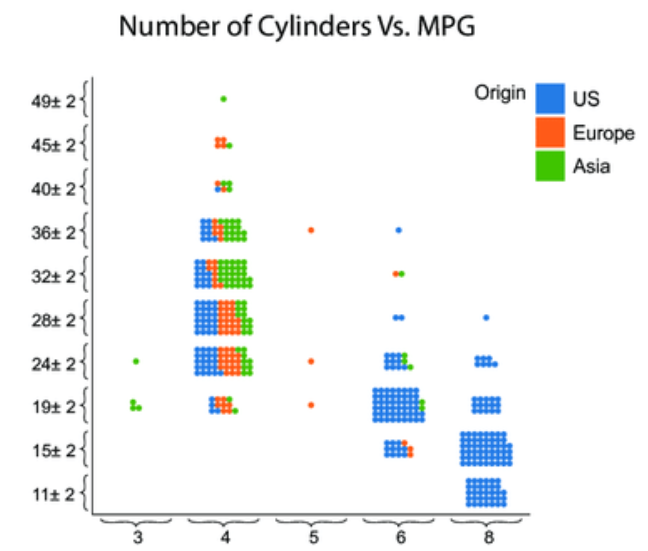
\includegraphics[width=\linewidth]{images/plots/independent/MPGbyCylinders.png} 
        \caption{\centering Milhas por galão por cilíndro.}
        \label{fig: MPGpCylinder}
    \end{minipage} \hfill
    \begin{minipage}[b]{0.45\textwidth}
        \centering
        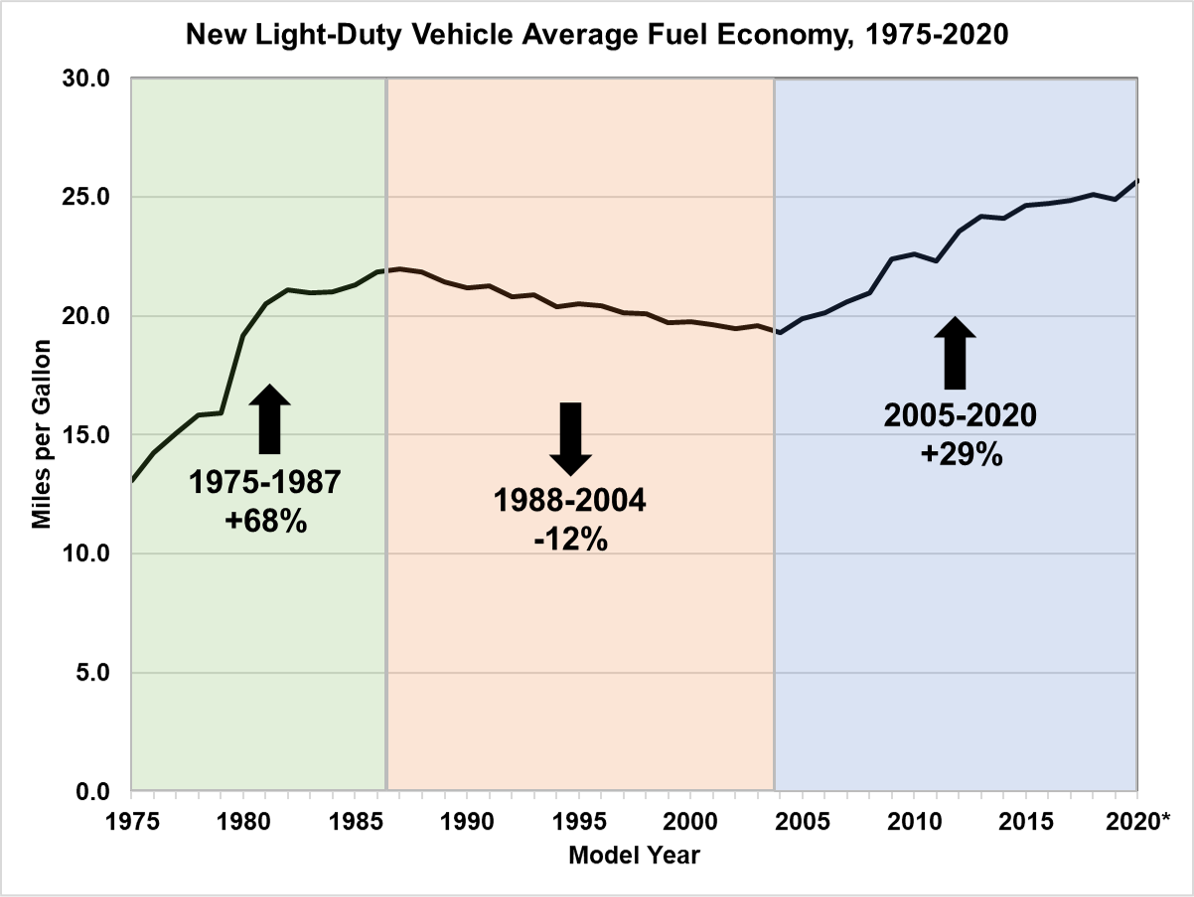
\includegraphics[width=\linewidth]{images/plots/independent/MPGbyYear.png}
        \caption{\centering Milhas por galão por ano}
        \label{fig: MPGbyYear}
    \end{minipage}
\end{figure}

O gráfico \ref{fig: MPGpCylinder} mostra que o consumo aumenta em média 4 milhas por galão a cada cilindro, enquanto o gráfico \ref{fig: MPGbyYear} mostra que em 15 anos, ocorreu um aumento de 30\% da eficiência dos combustíveis em carros, o que resulta em aproximadamente 0,5 milhas por galão ao ano, o que confirma os achados da regressão linear, onde o coeficiente atribuído ao número de cilindros é 8 vezes mais importante que o ano, portanto, enquanto a eficiência aumenta a cada ano, ela diminui a cada cilindro.

O deslocamento do carro tem uma relação direta com a quantidade de combustível utilizada, mas também com a quantidade de cilindros no carro, o que pode explicar o valor consideravelmente neutro que a variável teve.

A baixa importância dada aos atributos categóricos pode ser atribuída tanto à baixa correlação que existe entre estas variáveis independentes e a variável dependente, quanto devido ao modelo utilizado para juntar os coeficientes resultantes do \textit{One-Hot Encoder} ser imprópria, ou pelo grau da dimensionalidade que trazem para o problema, considerando que algumas categorias foram separadas em centenas pelo \textit{Encoder}, diminuindo sua relevância preditiva.
\section{Conclusões Finais}
Apesar do resultado ser satisfatório, a eficiência do preditor poderia ser melhorada utilizando estratificação no conjunto de treinamento, validação e teste, porém, o conjunto misto de dados numéricos e categóricos impediu o uso do parâmetro \textit{stratify} do \textit{train\_test\_split}, por tentar manter a distribuição de números raros e infrequentes das categorias numéricas nos conjuntos de treino e teste. A observabilidade poderia ser melhorada utilizando métodos para junção dos coeficientes categóricos mais adequados que a soma, como por exemplo, uma média ponderada de todos os coeficientes, ou um \textit{box plot} que demonstre o valor médio e o desvio de todos os coeficientes dentro de cada categoria.
Apesar destas dificuldades, o modelo de Regressão Linear mostrou-se muito capaz de adaptação ao problema de predição de consumo de combustível, apesar da sua simplicidade. Como visto na subseção \ref{subsec: analiseresultados}, o modelo é facilmente observável, permitindo afirmar que o modelo foi capaz de identificar padrões reais do problema utilizando somente as \textit{features} numéricas, classificando novos casos com precisão e superando modelos mais complexos e vulneráveis a \textit{overfitting}.


FAZER REFERENCIA DOS GRAFICOS, %https://www.researchgate.net/figure/Multiple-plots-showing-a-relation-between-the-number-of-cylinders-vs-gas-mileage-MPG_fig1_319328127
%https://www.energy.gov/eere/vehicles/articles/fotw-1177-march-15-2021-preliminary-data-show-average-fuel-economy-new-light
FAZER REFERENCIA DOS SITES DO SCIKIT LEARN QUE TIRAMOS OS PARAMETROS, SÃO OS DOIS ÚLTIMOS DA BIBLIOGRAFIA 


\clearpage
\printbibliography
\thispagestyle{empty}

\end{document}